\section{Sommes de \textsc{Riemann} généralisées}

\todoinline{
Alain : je supprimerai cette section en intégrant l'application probabiliste à la section sur la fonction Beta\\
Alain : j'ajouterais un thème sur l'approximation des intégrales.
}


\todoinline{Je pense que le cas "par morceaux" est pénible à montrer et peu utile. Se limiter à continue me semble suffisant.}

\begin{theo}{\textsc{Riemann}}
    \marginnote[0cm]{\cite{acamanes}}
    Pour tout entier naturel $n$ non nul, la \emph{somme de \textsc{Riemann}} associée à $f$ sur le segment $[a, b]$ est 
    $$S_n \defeq \frac{b-a}{n} \sum\limits_{k=0}^{n-1} f \left( a + k \frac{b-a}{n} \right).$$
    Si $f$ est continue par morceaux sur $[a, b]$, alors, 
    $$\lim_{n \to + \infty} S_n = \int_a^b f(t) \d t.$$
\end{theo}

%\begin{marginfigure}[-3cm]
%    %https://tex.stackexchange.com/questions/476702/riemann-sum-approaches-area-under-curve

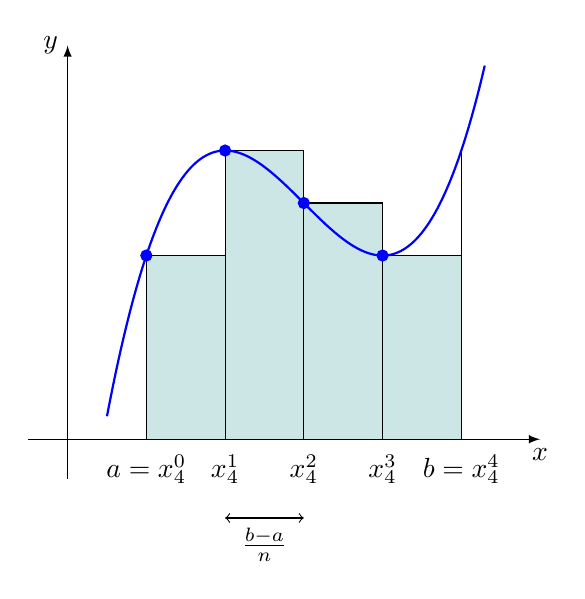
\begin{tikzpicture}[scale=1,declare function={f(\x)=((1/3)*(\x)^(3)-3*(\x)^(2)+8*\x-3;}]
\coordinate (start) at (.8,{f(.8)});
\coordinate (x0) at (1,{f(1)});
\coordinate (x1) at (2,{f(2)});
\coordinate (x2) at (3,{f(3)});
\coordinate (x3) at (4,{f(4)});
\coordinate (x4) at (5,{f(5)});
\coordinate (end) at (5.05,{f(5.05)});
\draw[fill=teal!20!white] (1,0) rectangle (2,{f(1)});
\draw[fill=teal!20!white] (2,0) rectangle (3,{f(2)});
\draw[fill=teal!20!white] (3,0) rectangle (4,{f(3)});
\draw[fill=teal!20!white] (4,0) rectangle (5,{f(4)});
\draw (5,0)--(5,{f(5)});
\draw [-latex] (-0.5,0) -- (6,0) node (xaxis) [below] {$x$};
\draw [-latex] (0,-0.5) -- (0,5) node [left] {$y$};
\foreach \x/\xtext in {1/a=x^0_{4} ,2/x^1_{4}, 3/x^2_{4} , 4/x^3_{4} , 5/b=x^4_{4}}
 \draw[xshift=\x cm] (0pt,3pt) -- (0pt,0pt) 
node[below=2pt,fill=white,font=\normalsize]
  {$\xtext$};
\draw[domain=.5:5.3,samples=200,variable=\x,blue,thick] plot ({\x},{f(\x)});                 
\foreach \n in {0,1,2,3}
\draw[blue,fill=blue] (x\n) circle (2pt) node[font=\normalsize] {$ $};    
\draw[<->] (2,-1)--(3,-1) node[below,midway] {$\frac{b-a}{n}$};      
\end{tikzpicture}
%\end{marginfigure}

\begin{preuve}
    
\end{preuve}

\todoinline{Je suis pas à fond pour l'exercice qui suit car c'est de l'application "bourrin". J'ai un exo avec une application en probabilités.}

\begin{exercice}
    \marginnote[0cm]{Source : \cite{maths-france} Planche no 37. Intégration sur un segment}
    Déterminer la limite quand $n$ tend vers $+ \infty$ des suites suivantes
    \setlength{\columnseprule}{0pt}
    \begin{multicols}{2}
        \begin{enumerate}
            \item $$\frac{1}{n^3} \sum_{k=1}^n k^2 \sin \frac{k \pi}{n}$$
            \item Soit $a > 0$, 
            $$\left( \frac{1}{n!} \prod_{k=1}^n (a+k) \right)^{1/n}$$
            \item $$\sum_{k=1}^n \frac{n+k}{n^2+k}$$
            \item $$\sum_{k=0}^{n-1} \frac{1}{\sqrt{n^2-k^2}}$$
            \item $$\frac{1}{n \sqrt{n}} \sum_{k=1}^n \left \lfloor \sqrt{k} \right \rfloor$$
            \item $$\sum_{k=1}^n \frac{k^2}{8k^3 + n^3}$$
            \item $$\sum_{k=n}^{2n-1} \frac{1}{2k+1}$$
            \item $$n \sum_{k=1}^n \frac{\e^{-n/k}}{k^2}$$
        \end{enumerate}
    \end{multicols}
\end{exercice}

\begin{solution}
    \begin{enumerate}
        \item 
    \end{enumerate}
\end{solution}

\begin{methode}
    \begin{itemize}
        \item 
    \end{itemize}
\end{methode}



%---------------

\todoinline{On peut aussi le mettre dans un chapitre sur la fonction Beta. Je crois pas que ce soit la même chose que le renforcement de Polya qui converge vers une loi Beta, mais il faut regarder plus en détail pour être sûr (si on garde).}

\begin{exercice}%
{RMS 2017 1071 \& 1073}%
{Centrale 16'}%
\begin{enumerate}
\item Soit $(p, q) \in (\N^\ast)^2$. Calculer l'intégrale $\int_0^1 x^p (1 - x)^q \d x$.

\item Soit $p \in \N^\ast$. On dispose de $p$ urnes numérotées de $1$ à $p$. Chaque urne contient $p$ boules et pour tout $i \in \entiers{1}{p}$, l'urne numéro $i$ contient $i$ boules noires et $p - i$ boules blanches. On effectue l'expérience suivante : choisir au hasard une urne puis effectuer des tirages avec remise dans l'urne choisie. On note, pour $n \in \N^\ast$, $A_n$ l'événement \textit{on a effectué $2 n$ tirages et obtenu le même nombre de boules blanches que de noires}.
\begin{itemize}
\item Exprimer $\mathbf{P}(A_n)$ sous forme d'une somme.

\item On note $b_{n,p}$ la probabilité que la prochaine boule tirée soit blanche sachant que $A_n$ est réalisé. Exprimer $b_{n,p}$.
\item Calculer $\lim\limits_{p\to+\infty} b_{n,p}$.
\end{itemize}
\end{enumerate}
\end{exercice}

\begin{preuve}
\begin{itemize}
\item En effectuant une intégration par parties, dès que $q > 0$, alors $I_{p,q} = \frac{q}{p+1} I_{p+1, q-1}$. Ainsi, par récurrence,
\[
I_{p,q} = \prod_{k=0}^{q-1} \frac{q - k}{p+1+k} I_{p+q, 0} = \frac{q! p!}{(p+q+1)!}.
\]

\item
\begin{itemize}
\item En utilisant la formule des probabilités totales,
\begin{align*}
\mathbf{P}(A_n) &= \sum_{i=1}^p \mathbf{P}(A_n | U_i) \mathbf{P}(U_i) \\
&= \sum_{i=1}^n \binom{2n}{n} \left(\frac{p-i}{p}\right)^n \left(\frac{i}{p}\right)^n.
\end{align*}

\item En utilisant le même raisonnement que précédemment,
\[
b_{n,p} = \frac{\frac{1}{p} \sum_{i=1}^p \left(1 - \frac{i}{p}\right)^{n+1} \left(\frac{i}{p}\right)^n}{\frac{1}{p} \sum_{i=1}^p \left(1 - \frac{i}{p}\right)^{n} \left(\frac{i}{p}\right)^n} \cdot \frac{\binom{2n+1}{n+1}}{\binom{2n}{n}}.
\]

\item En utilisant les limites des sommes de Riemann,
\[
\lim\limits_{p\to+\infty} b_{n,p} = \frac{2n+1}{n+1} \cdot \frac{\int_0^1 (1 - x)^{n+1} x^n \d x}{\int_0^1 (1 - x)^n x^n \d x}.
\]
Cette limite vaut donc
\[
\frac{2n+1}{n+1} \cdot \frac{n! (n+1)!}{(2n+2)!} \cdot \frac{(2n+1)!}{n! n!}  = \frac{2n+1}{2n+2}.
\]
\end{itemize}
\end{itemize}
\end{preuve}


\todoinline{Je mettrais plutôt un thème sur les calculs approchés d'intégrales : rectangles gauche, médian, trapèze, Simpson ?}

Les sommes de \textsc{Riemann} permettent de calculer des intégrales mais leur convergence est lente comme le montre l'exercice suivant.

\begin{exercice}
    \marginnote[0cm]{Source : \cite{maths-france} Planche no 37. Intégration sur un segment}
    Soit $f$ une fonction de classe $\mathscr{C}^2$ sur $[0, 1]$. Déterminer le réel $a$ tel que:
    $$\int_0^1 f(t) \d t - \frac{1}{n} \sum_{k=1}^{n-1} f \left( \frac{k}{n} \right) =\lim\limits_{n \to + \infty} \frac{a}{n} + o \left( \frac{1}{n} \right).$$
    \end{exercice}